\documentclass[aspectratio=169]{beamer}
\usepackage{standalone}

\usepackage{stmaryrd}
\usepackage{listings}
\usepackage{bussproofs}

\usepackage[hyperref=auto,style=alphabetic,backend=bibtex]{biblatex}
\addbibresource{kwarcpubs.bib}
\addbibresource{extpubs.bib}
\addbibresource{extcrossrefs.bib}
\addbibresource{bib.bib}
\usepackage{appendixnumberbeamer}
\usepackage{tikz}
\usepackage{tikz-qtree}
\usetikzlibrary{arrows.meta}
\usetikzlibrary{shapes}
\usetikzlibrary{mmt}
\usetikzlibrary{docicon}

\usetheme{Pittsburgh}
% \setbeamertemplate{footline}[frame number]
\setbeamertemplate{footline}{\hfill\insertframenumber\,/\,\inserttotalframenumber\quad\strut}
\setbeamertemplate{navigation symbols}{}
\usecolortheme{beaver}
\setbeamertemplate{frametitle}[default][left]
% \setbeamersize{text margin left=3em}

\usepackage{utils/colors}
\usepackage[forbeamer]{utils/basic}
\usepackage{utils/operators}
\usepackage{utils/mylstmisc}
\usepackage{utils/lstmmt}

\lstset{basicstyle=\ttfamily}
\lstset{commentstyle=\itshape\color{commentfont}}

\title{Towards and Annotation Standard for STEM Documents \\\large Datasets, Benchmarks, and Spotters}


% rdf nodes
\tikzset{urinode/.style={draw, ellipse, minimum width=1.3cm, minimum height=0.6cm}}
\tikzset{typenode/.style={draw}}
\tikzset{bnode/.style={draw, ellipse, minimum width=1.0cm, minimum height=0.6cm}}
\tikzset{literal/.style={draw, rounded corners=0.1cm}}

% rdf edges
\tikzset{normaledge/.style={-Latex}}
\tikzset{typeedge/.style={arrows={-Latex[open]}}}

% custom nodes
\tikzset{body/.style={fill=green!50}}
\tikzset{target/.style={fill=blue!50}}
\tikzset{annotation/.style={fill=red!50}}


\author{\textbf{Jan Frederik Schaefer} \and Michael Kohlhase}
\institute{FAU Erlangen-N\"urnberg/KWARC}
\date{\textbf{Conference on Intelligent Computer Mathematics (CICM)}\\Cambridge, UK\\September 7, 2023}

\begin{document}
\frame\titlepage


\begin{frame}
    \frametitle{Motivation: semantic services}
    \begin{itemize}
        \item Computable formulae
        \item Screen readers
        \item Active documents
        \item Formula search
    \end{itemize}
\end{frame}


\begin{frame}
    \frametitle{We need semantic annotations!}
    % example picture with annotations
\end{frame}


\begin{frame}
    \frametitle{Accumulating semantic annotations with spotters}
    \begin{itemize}
        \item \textbf{Spotter:} specialized tool for finding a particular type of annotation
        \item Examples: Identifier declarations, quantity expressions,
            paragraph type (theorem/definition/\textellipsis), \textellipsis
        \item Simple spotters, hybrid spotters, meta spotters
    \end{itemize}
    % pictures with annotations (simple spotter, hybrid spotter, meta spotter)
    % e.g. "concept references and quantities", "variable declarations", "conflict resolution var. occurrence vs unit"
\end{frame}


\begin{frame}
    \frametitle{What is the problem?}
    \begin{enumerate}
        \item Getting a corpus:\com{Working with PDF is difficult}
            \begin{itemize}
                \item arXMLiv/ar5iv dataset\com{convert \texttt{.tex} to \texttt{.html}}
                \item SIGMathLing\com{NDA-cooperative to work around licensing issues}
            \end{itemize}
        \item Re-inventing the wheel:
            \begin{itemize}
                \item Need to obtain plaintext representation
                \item Need to store annotations
                \item Need to create manual annotations\com{for training/evaluation}
            \end{itemize}
        \item Cannot re-use existing annotations/combine results:
            \begin{itemize}
                \item No agreed-upon annotation format
                \item Original documents modified
            \end{itemize}
    \end{enumerate}
\end{frame}


\begin{frame}
    \frametitle{A new annotation standard}
    \begin{itemize}
        \item Supports development of re-usable tools, datasets and benchmarks
        \item Uses RDF (Resource Description Framework)\com{$\exists$ databases, query language (SPARQL), serialization formats}
        \item Based on W3C Web Annotation Standard
    \end{itemize}
    % based on RDF, Web Annotation Standard, ...
    \pause
    \vspace{1.5em}
    \rule{\textwidth}{0.4pt}\\
    \vspace{1.5em}
    \textbf{RDF Primer}\\[1em]
    \begin{tabular}{ll}
        subject-predicate-object triple\quad\quad\quad &
        \texttt{ex:anno1 rdf:type oa:Annotation} \\[1em]
        directed graph &
        \begin{tikzpicture}[baseline={([yshift=-.5ex]current bounding box.center)}]
            \node[urinode] (s) at (0, 0) {{ex:anno1}};
            \node[urinode] (o) at (4.5, 0) {{oa:Annotation}};
            \draw[normaledge] (s) --node[above]{{rdf:type}} (o);
        \end{tikzpicture}\\
    \end{tabular}
\end{frame}


\begin{frame}
    \frametitle{Annotation structure (following W3C Web Annotation Recommendation)}
    \centering
    % body, target, meta-data
    \begin{tikzpicture}[yscale=1.8]
        \node[urinode,annotation] (anno) at (0, 0) {ex:anno1};
        
        \node[typenode] (annot) at (-4.5, 1) {oa:Annotation};
        \draw[typeedge] (anno) --node[fill=white]{rdf:type} (annot);
        \node[urinode] (author) at (0, 1) {\textellipsis};
        \draw[normaledge] (anno) --node[fill=white,pos=0.4]{dcterms:creator} (author);
        \node[urinode] (created) at (4.5, 1) {\textellipsis};
        \draw[normaledge] (anno) --node[fill=white,pos=0.6]{dcterms:created} (created);

        \pause
        \node (targ) at (-3, -1) {\textellipsis};
        \draw[normaledge] (anno) --node[fill=white]{oa:hasTarget} (targ);
        % \node[urinode] (targ) at (-3, -1) {ex:target1};
        % \draw[normaledge] (anno) --node[fill=white]{oa:hasTarget} (targ);
        % \node (targ1) at (-4,-1.5) {\textellipsis};
        % \node (targ2) at (-2,-1.5) {\textellipsis};
        % \draw[normaledge] (targ) -- (targ1);
        % \draw[normaledge] (targ) -- (targ2);

        % \node[urinode] (body) at (3,-1) {ex:body1};
        \node (body) at (3,-1) {\textellipsis};
        \draw[normaledge] (anno) --node[fill=white]{oa:hasBody} (body);
    \end{tikzpicture}
    \pause
    \vspace{2em}\par
    \begin{columns}
        \begin{column}{0.5\textwidth}
            \centering
            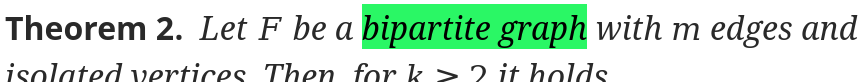
\includegraphics[width=\textwidth]{bipart_graph.png}
        \end{column}
        \begin{column}{0.5\textwidth}
            \centering
            \texttt{wd:Q174733}\\
            (WikiData: bipartite graph)
        \end{column}
    \end{columns}
\end{frame}


\begin{frame}
    \frametitle{Example annotation bodies: simple annotation}
    \centering
    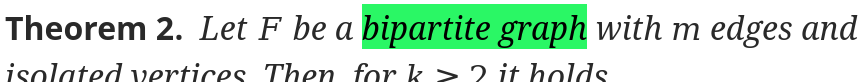
\includegraphics[width=0.8\textwidth]{bipart_graph.png}
    \par
    \begin{tikzpicture}
        \node[urinode,annotation] (anno) at (0, 2) {ex:anno1};
        \node[urinode,body] (bipart_graph) at (0, 0) {wd:Q174733};
        \node (target) at (0, 4) {};
        \draw[normaledge] (anno) --node[fill=white]{oa:hasBody} (bipart_graph);
        \draw[normaledge] (anno) --node[fill=white]{oa:hasTarget} (target);
        \pause
        \node[urinode,black!70] (multipartgraph) at (-4, 1.5) {wd:Q1718082};
        \draw[normaledge,black!70] (bipart_graph) --node[fill=white]{subclass of} (multipartgraph);
        \node[literal,black!70] (labelfr) at (4, 1.5) {``graphe biparti''\makeatletter @\makeatother fr};
        \node[literal,black!70] (labelde) at (4, -1.5) {``bipartiter Graph''\makeatletter @\makeatother de};
        \draw[normaledge,black!70] (bipart_graph) --node[fill=white]{rdfs:label} (labelfr);
        \draw[normaledge,black!70] (bipart_graph) --node[fill=white]{rdfs:label} (labelde);
        \node[urinode,black!70] (graphtheo) at (-3.5, -1.5) {wd:Q131476};
        \draw[normaledge,black!70] (bipart_graph) --node[fill=white]{studied by} (graphtheo);
        \node[black!70] (dots1) at (-5.5, 0.6) {\textellipsis};
        \draw[normaledge,black!70] (multipartgraph) -- (dots1);
        \node[black!70] (dots2) at (-5.1, -0.5) {\textellipsis};
        \draw[normaledge,black!70] (graphtheo) -- (dots2);
        \node[black!70] (dots3) at (-0.5, -1.7) {\textellipsis};
        \draw[normaledge,black!70] (graphtheo) -- (dots3);
    \end{tikzpicture}
\end{frame}

\begin{frame}
    \frametitle{Example annotation bodies: complex body}
    \centering
    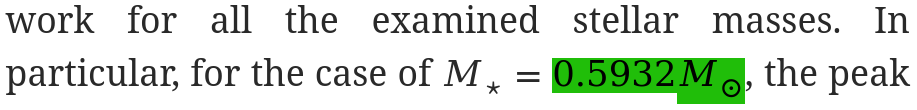
\includegraphics[width=0.7\textwidth]{solarmass_2205_14126.png}
    \par
    \begin{tikzpicture}
        \node[urinode,annotation] (anno) at (0, 2) {ex:anno2};
        \node[bnode,body] (body) at (0, 0) {};
        \node (target) at (0, 4) {};
        \draw[normaledge] (anno) --node[fill=white]{oa:hasBody} (bipart_graph);
        \draw[normaledge] (anno) --node[fill=white]{oa:hasTarget} (target);
        \node[typenode,body] (measure) at (-4, 1.7) {om:Measure};
        \node[literal,body] (scalar) at (-3, -1.7) {0.5932};
        \node[urinode,body] (unit) at (3.5, -1.7) {om:solarMass};
        \draw[normaledge] (body) --node[fill=white]{rdf:type} (measure);
        \draw[normaledge] (body) --node[fill=white]{om:hasNumericalValue} (scalar);
        \draw[normaledge] (body) --node[fill=white]{om:hasUnit} (unit);
        \node[urinode,black!70] (dim) at (5, 0) {om:mass-Dimension};
        \draw[normaledge,black!70] (unit) --node[fill=white]{om:hasDimension} (dim);
    \end{tikzpicture}
\end{frame}

\begin{frame}
    \frametitle{Example annotation bodies: linked bodies}

\end{frame}


\begin{frame}
    \frametitle{Annotation Targets}
\end{frame}


\begin{frame}
    \frametitle{Prototype datasets and imported datasets}
\end{frame}


\begin{frame}
    \frametitle{Querying}
\end{frame}


\begin{frame}
    \frametitle{Adoption}
    % Concern   ->   answer
    % No datasets exist - what do I get concretely?    ->   annotation tool
    % I don't know RDF/can't use it in my environment   ->   JSON-LD
    % But I need dataset XYZ in a different format   ->   conversion?
\end{frame}


\begin{frame}
    \frametitle{Conclusion}
\end{frame}

\begin{frame}
\end{frame}


\begin{frame}[allowframebreaks,t]
    \frametitle{References}
    \printbibliography
\end{frame}

\end{document}
